% Created by tikzDevice version 0.10.1 on 2016-09-05 22:30:08
% !TEX encoding = UTF-8 Unicode
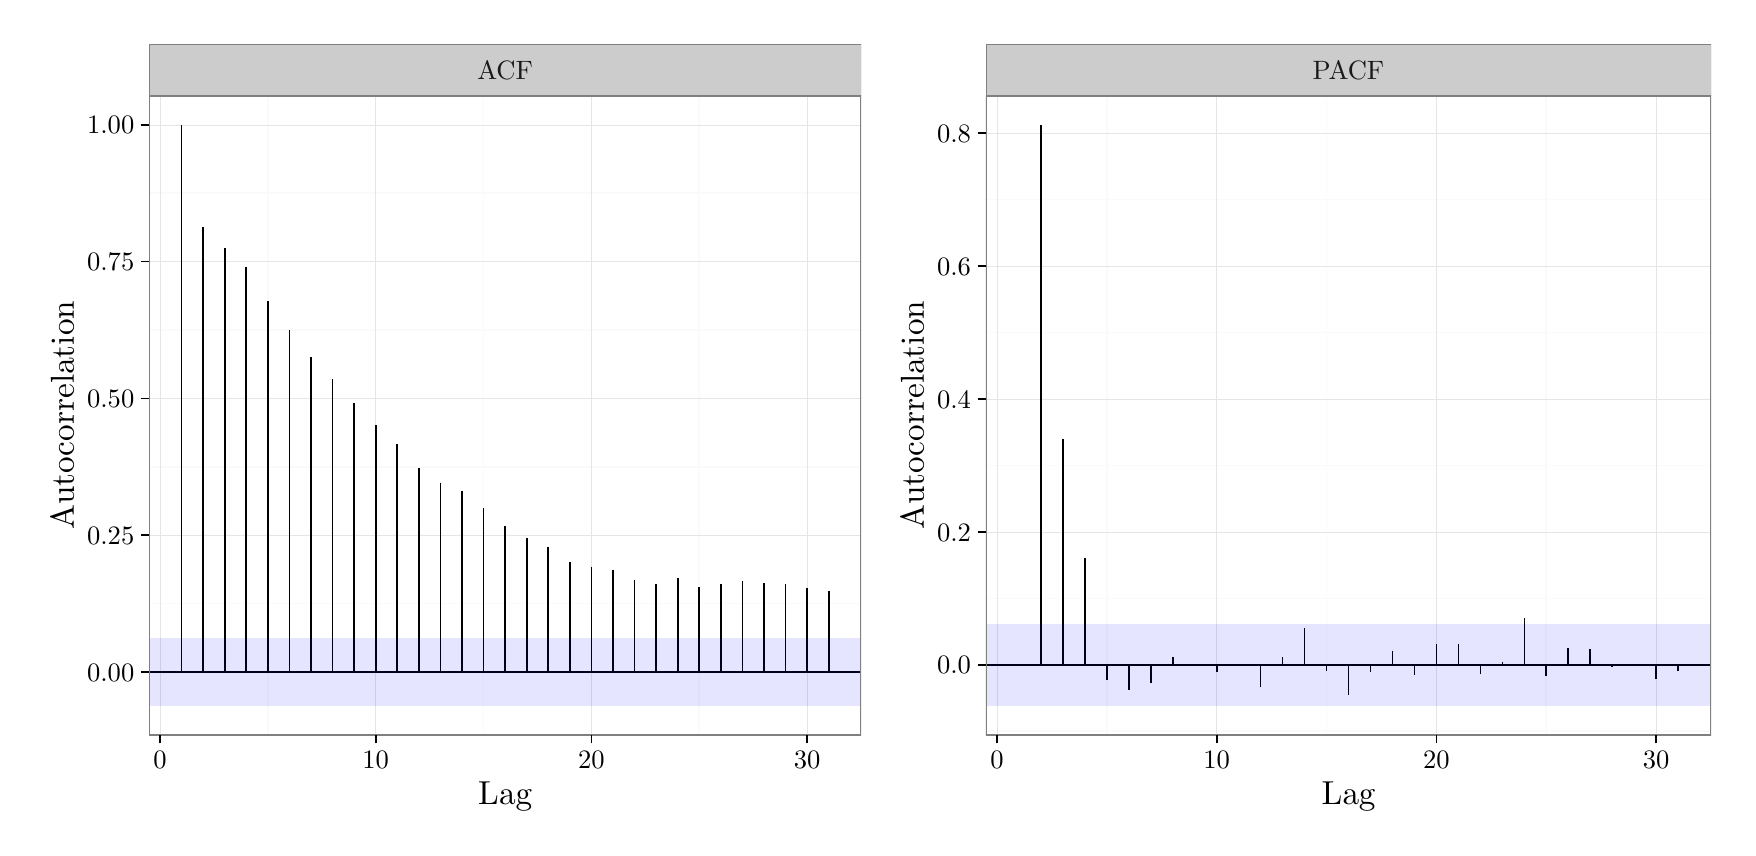
\begin{tikzpicture}[x=1pt,y=1pt]
\definecolor{fillColor}{RGB}{255,255,255}
\path[use as bounding box,fill=fillColor,fill opacity=0.00] (0,0) rectangle (614.29,289.08);
\begin{scope}
\path[clip] (  0.00,  0.00) rectangle (307.15,289.08);
\definecolor{drawColor}{RGB}{255,255,255}
\definecolor{fillColor}{RGB}{255,255,255}

\path[draw=drawColor,line width= 0.6pt,line join=round,line cap=round,fill=fillColor] ( -0.00,  0.00) rectangle (307.15,289.08);
\end{scope}
\begin{scope}
\path[clip] ( 43.93, 33.48) rectangle (301.15,264.47);
\definecolor{fillColor}{RGB}{255,255,255}

\path[fill=fillColor] ( 43.93, 33.48) rectangle (301.15,264.47);
\definecolor{drawColor}{gray}{0.98}

\path[draw=drawColor,line width= 0.6pt,line join=round] ( 43.93, 80.95) --
	(301.15, 80.95);

\path[draw=drawColor,line width= 0.6pt,line join=round] ( 43.93,130.38) --
	(301.15,130.38);

\path[draw=drawColor,line width= 0.6pt,line join=round] ( 43.93,179.82) --
	(301.15,179.82);

\path[draw=drawColor,line width= 0.6pt,line join=round] ( 43.93,229.25) --
	(301.15,229.25);

\path[draw=drawColor,line width= 0.6pt,line join=round] ( 86.80, 33.48) --
	( 86.80,264.47);

\path[draw=drawColor,line width= 0.6pt,line join=round] (164.74, 33.48) --
	(164.74,264.47);

\path[draw=drawColor,line width= 0.6pt,line join=round] (242.69, 33.48) --
	(242.69,264.47);
\definecolor{drawColor}{gray}{0.90}

\path[draw=drawColor,line width= 0.2pt,line join=round] ( 43.93, 56.23) --
	(301.15, 56.23);

\path[draw=drawColor,line width= 0.2pt,line join=round] ( 43.93,105.67) --
	(301.15,105.67);

\path[draw=drawColor,line width= 0.2pt,line join=round] ( 43.93,155.10) --
	(301.15,155.10);

\path[draw=drawColor,line width= 0.2pt,line join=round] ( 43.93,204.53) --
	(301.15,204.53);

\path[draw=drawColor,line width= 0.2pt,line join=round] ( 43.93,253.97) --
	(301.15,253.97);

\path[draw=drawColor,line width= 0.2pt,line join=round] ( 47.82, 33.48) --
	( 47.82,264.47);

\path[draw=drawColor,line width= 0.2pt,line join=round] (125.77, 33.48) --
	(125.77,264.47);

\path[draw=drawColor,line width= 0.2pt,line join=round] (203.72, 33.48) --
	(203.72,264.47);

\path[draw=drawColor,line width= 0.2pt,line join=round] (281.66, 33.48) --
	(281.66,264.47);
\definecolor{drawColor}{RGB}{0,0,0}

\path[draw=drawColor,line width= 0.6pt,line join=round] ( 43.93, 56.23) -- (301.15, 56.23);

\path[draw=drawColor,line width= 0.6pt,line join=round] ( 55.62,253.97) -- ( 55.62, 56.23);

\path[draw=drawColor,line width= 0.6pt,line join=round] ( 63.41,216.90) -- ( 63.41, 56.23);

\path[draw=drawColor,line width= 0.6pt,line join=round] ( 71.21,209.63) -- ( 71.21, 56.23);

\path[draw=drawColor,line width= 0.6pt,line join=round] ( 79.00,202.71) -- ( 79.00, 56.23);

\path[draw=drawColor,line width= 0.6pt,line join=round] ( 86.80,190.25) -- ( 86.80, 56.23);

\path[draw=drawColor,line width= 0.6pt,line join=round] ( 94.59,179.82) -- ( 94.59, 56.23);

\path[draw=drawColor,line width= 0.6pt,line join=round] (102.39,170.01) -- (102.39, 56.23);

\path[draw=drawColor,line width= 0.6pt,line join=round] (110.18,162.02) -- (110.18, 56.23);

\path[draw=drawColor,line width= 0.6pt,line join=round] (117.98,153.60) -- (117.98, 56.23);

\path[draw=drawColor,line width= 0.6pt,line join=round] (125.77,145.40) -- (125.77, 56.23);

\path[draw=drawColor,line width= 0.6pt,line join=round] (133.56,138.59) -- (133.56, 56.23);

\path[draw=drawColor,line width= 0.6pt,line join=round] (141.36,130.06) -- (141.36, 56.23);

\path[draw=drawColor,line width= 0.6pt,line join=round] (149.15,124.65) -- (149.15, 56.23);

\path[draw=drawColor,line width= 0.6pt,line join=round] (156.95,121.68) -- (156.95, 56.23);

\path[draw=drawColor,line width= 0.6pt,line join=round] (164.74,115.38) -- (164.74, 56.23);

\path[draw=drawColor,line width= 0.6pt,line join=round] (172.54,108.84) -- (172.54, 56.23);

\path[draw=drawColor,line width= 0.6pt,line join=round] (180.33,104.72) -- (180.33, 56.23);

\path[draw=drawColor,line width= 0.6pt,line join=round] (188.13,101.49) -- (188.13, 56.23);

\path[draw=drawColor,line width= 0.6pt,line join=round] (195.92, 96.03) -- (195.92, 56.23);

\path[draw=drawColor,line width= 0.6pt,line join=round] (203.72, 94.33) -- (203.72, 56.23);

\path[draw=drawColor,line width= 0.6pt,line join=round] (211.51, 92.96) -- (211.51, 56.23);

\path[draw=drawColor,line width= 0.6pt,line join=round] (219.30, 89.39) -- (219.30, 56.23);

\path[draw=drawColor,line width= 0.6pt,line join=round] (227.10, 88.02) -- (227.10, 56.23);

\path[draw=drawColor,line width= 0.6pt,line join=round] (234.89, 90.19) -- (234.89, 56.23);

\path[draw=drawColor,line width= 0.6pt,line join=round] (242.69, 87.00) -- (242.69, 56.23);

\path[draw=drawColor,line width= 0.6pt,line join=round] (250.48, 87.91) -- (250.48, 56.23);

\path[draw=drawColor,line width= 0.6pt,line join=round] (258.28, 89.08) -- (258.28, 56.23);

\path[draw=drawColor,line width= 0.6pt,line join=round] (266.07, 88.33) -- (266.07, 56.23);

\path[draw=drawColor,line width= 0.6pt,line join=round] (273.87, 87.96) -- (273.87, 56.23);

\path[draw=drawColor,line width= 0.6pt,line join=round] (281.66, 86.50) -- (281.66, 56.23);

\path[draw=drawColor,line width= 0.6pt,line join=round] (289.46, 85.68) -- (289.46, 56.23);
\definecolor{fillColor}{RGB}{0,0,255}

\path[fill=fillColor,fill opacity=0.10] ( 43.93, 43.98) rectangle (301.15, 68.49);
\definecolor{drawColor}{gray}{0.50}

\path[draw=drawColor,line width= 0.6pt,line join=round,line cap=round] ( 43.93, 33.48) rectangle (301.15,264.47);
\end{scope}
\begin{scope}
\path[clip] ( 43.93,264.47) rectangle (301.15,283.08);
\definecolor{drawColor}{gray}{0.50}
\definecolor{fillColor}{gray}{0.80}

\path[draw=drawColor,line width= 0.2pt,line join=round,line cap=round,fill=fillColor] ( 43.93,264.47) rectangle (301.15,283.08);
\definecolor{drawColor}{gray}{0.10}

\node[text=drawColor,anchor=base,inner sep=0pt, outer sep=0pt, scale=  0.96] at (172.54,270.47) {ACF};
\end{scope}
\begin{scope}
\path[clip] (  0.00,  0.00) rectangle (614.29,289.08);
\definecolor{drawColor}{RGB}{0,0,0}

\node[text=drawColor,anchor=base east,inner sep=0pt, outer sep=0pt, scale=  0.96] at ( 38.53, 52.93) {0.00};

\node[text=drawColor,anchor=base east,inner sep=0pt, outer sep=0pt, scale=  0.96] at ( 38.53,102.36) {0.25};

\node[text=drawColor,anchor=base east,inner sep=0pt, outer sep=0pt, scale=  0.96] at ( 38.53,151.79) {0.50};

\node[text=drawColor,anchor=base east,inner sep=0pt, outer sep=0pt, scale=  0.96] at ( 38.53,201.23) {0.75};

\node[text=drawColor,anchor=base east,inner sep=0pt, outer sep=0pt, scale=  0.96] at ( 38.53,250.66) {1.00};
\end{scope}
\begin{scope}
\path[clip] (  0.00,  0.00) rectangle (614.29,289.08);
\definecolor{drawColor}{RGB}{0,0,0}

\path[draw=drawColor,line width= 0.6pt,line join=round] ( 40.93, 56.23) --
	( 43.93, 56.23);

\path[draw=drawColor,line width= 0.6pt,line join=round] ( 40.93,105.67) --
	( 43.93,105.67);

\path[draw=drawColor,line width= 0.6pt,line join=round] ( 40.93,155.10) --
	( 43.93,155.10);

\path[draw=drawColor,line width= 0.6pt,line join=round] ( 40.93,204.53) --
	( 43.93,204.53);

\path[draw=drawColor,line width= 0.6pt,line join=round] ( 40.93,253.97) --
	( 43.93,253.97);
\end{scope}
\begin{scope}
\path[clip] (  0.00,  0.00) rectangle (614.29,289.08);
\definecolor{drawColor}{RGB}{0,0,0}

\path[draw=drawColor,line width= 0.6pt,line join=round] ( 47.82, 30.48) --
	( 47.82, 33.48);

\path[draw=drawColor,line width= 0.6pt,line join=round] (125.77, 30.48) --
	(125.77, 33.48);

\path[draw=drawColor,line width= 0.6pt,line join=round] (203.72, 30.48) --
	(203.72, 33.48);

\path[draw=drawColor,line width= 0.6pt,line join=round] (281.66, 30.48) --
	(281.66, 33.48);
\end{scope}
\begin{scope}
\path[clip] (  0.00,  0.00) rectangle (614.29,289.08);
\definecolor{drawColor}{RGB}{0,0,0}

\node[text=drawColor,anchor=base,inner sep=0pt, outer sep=0pt, scale=  0.96] at ( 47.82, 21.46) {0};

\node[text=drawColor,anchor=base,inner sep=0pt, outer sep=0pt, scale=  0.96] at (125.77, 21.46) {10};

\node[text=drawColor,anchor=base,inner sep=0pt, outer sep=0pt, scale=  0.96] at (203.72, 21.46) {20};

\node[text=drawColor,anchor=base,inner sep=0pt, outer sep=0pt, scale=  0.96] at (281.66, 21.46) {30};
\end{scope}
\begin{scope}
\path[clip] (  0.00,  0.00) rectangle (614.29,289.08);
\definecolor{drawColor}{RGB}{0,0,0}

\node[text=drawColor,anchor=base,inner sep=0pt, outer sep=0pt, scale=  1.20] at (172.54,  8.40) {Lag};
\end{scope}
\begin{scope}
\path[clip] (  0.00,  0.00) rectangle (614.29,289.08);
\definecolor{drawColor}{RGB}{0,0,0}

\node[text=drawColor,rotate= 90.00,anchor=base,inner sep=0pt, outer sep=0pt, scale=  1.20] at ( 16.66,148.97) {Autocorrelation};
\end{scope}
\begin{scope}
\path[clip] (307.15,  0.00) rectangle (614.29,289.08);
\definecolor{drawColor}{RGB}{255,255,255}
\definecolor{fillColor}{RGB}{255,255,255}

\path[draw=drawColor,line width= 0.6pt,line join=round,line cap=round,fill=fillColor] (307.15,  0.00) rectangle (614.29,289.08);
\end{scope}
\begin{scope}
\path[clip] (346.28, 33.48) rectangle (608.30,264.47);
\definecolor{fillColor}{RGB}{255,255,255}

\path[fill=fillColor] (346.28, 33.48) rectangle (608.29,264.47);
\definecolor{drawColor}{gray}{0.98}

\path[draw=drawColor,line width= 0.6pt,line join=round] (346.28, 34.85) --
	(608.30, 34.85);

\path[draw=drawColor,line width= 0.6pt,line join=round] (346.28, 82.87) --
	(608.30, 82.87);

\path[draw=drawColor,line width= 0.6pt,line join=round] (346.28,130.90) --
	(608.30,130.90);

\path[draw=drawColor,line width= 0.6pt,line join=round] (346.28,178.92) --
	(608.30,178.92);

\path[draw=drawColor,line width= 0.6pt,line join=round] (346.28,226.95) --
	(608.30,226.95);

\path[draw=drawColor,line width= 0.6pt,line join=round] (389.95, 33.48) --
	(389.95,264.47);

\path[draw=drawColor,line width= 0.6pt,line join=round] (469.35, 33.48) --
	(469.35,264.47);

\path[draw=drawColor,line width= 0.6pt,line join=round] (548.75, 33.48) --
	(548.75,264.47);
\definecolor{drawColor}{gray}{0.90}

\path[draw=drawColor,line width= 0.2pt,line join=round] (346.28, 58.86) --
	(608.30, 58.86);

\path[draw=drawColor,line width= 0.2pt,line join=round] (346.28,106.89) --
	(608.30,106.89);

\path[draw=drawColor,line width= 0.2pt,line join=round] (346.28,154.91) --
	(608.30,154.91);

\path[draw=drawColor,line width= 0.2pt,line join=round] (346.28,202.94) --
	(608.30,202.94);

\path[draw=drawColor,line width= 0.2pt,line join=round] (346.28,250.96) --
	(608.30,250.96);

\path[draw=drawColor,line width= 0.2pt,line join=round] (350.25, 33.48) --
	(350.25,264.47);

\path[draw=drawColor,line width= 0.2pt,line join=round] (429.65, 33.48) --
	(429.65,264.47);

\path[draw=drawColor,line width= 0.2pt,line join=round] (509.05, 33.48) --
	(509.05,264.47);

\path[draw=drawColor,line width= 0.2pt,line join=round] (588.45, 33.48) --
	(588.45,264.47);
\definecolor{drawColor}{RGB}{0,0,0}

\path[draw=drawColor,line width= 0.6pt,line join=round] (346.28, 58.86) -- (608.30, 58.86);

\path[draw=drawColor,line width= 0.6pt,line join=round] (366.13,253.97) -- (366.13, 58.86);

\path[draw=drawColor,line width= 0.6pt,line join=round] (374.07,140.53) -- (374.07, 58.86);

\path[draw=drawColor,line width= 0.6pt,line join=round] (382.01, 97.62) -- (382.01, 58.86);

\path[draw=drawColor,line width= 0.6pt,line join=round] (389.95, 53.46) -- (389.95, 58.86);

\path[draw=drawColor,line width= 0.6pt,line join=round] (397.89, 49.79) -- (397.89, 58.86);

\path[draw=drawColor,line width= 0.6pt,line join=round] (405.83, 52.15) -- (405.83, 58.86);

\path[draw=drawColor,line width= 0.6pt,line join=round] (413.77, 61.59) -- (413.77, 58.86);

\path[draw=drawColor,line width= 0.6pt,line join=round] (421.71, 58.89) -- (421.71, 58.86);

\path[draw=drawColor,line width= 0.6pt,line join=round] (429.65, 56.20) -- (429.65, 58.86);

\path[draw=drawColor,line width= 0.6pt,line join=round] (437.59, 58.60) -- (437.59, 58.86);

\path[draw=drawColor,line width= 0.6pt,line join=round] (445.53, 50.68) -- (445.53, 58.86);

\path[draw=drawColor,line width= 0.6pt,line join=round] (453.47, 61.60) -- (453.47, 58.86);

\path[draw=drawColor,line width= 0.6pt,line join=round] (461.41, 71.98) -- (461.41, 58.86);

\path[draw=drawColor,line width= 0.6pt,line join=round] (469.35, 56.63) -- (469.35, 58.86);

\path[draw=drawColor,line width= 0.6pt,line join=round] (477.29, 48.09) -- (477.29, 58.86);

\path[draw=drawColor,line width= 0.6pt,line join=round] (485.23, 56.20) -- (485.23, 58.86);

\path[draw=drawColor,line width= 0.6pt,line join=round] (493.17, 63.92) -- (493.17, 58.86);

\path[draw=drawColor,line width= 0.6pt,line join=round] (501.11, 55.19) -- (501.11, 58.86);

\path[draw=drawColor,line width= 0.6pt,line join=round] (509.05, 66.51) -- (509.05, 58.86);

\path[draw=drawColor,line width= 0.6pt,line join=round] (516.99, 66.47) -- (516.99, 58.86);

\path[draw=drawColor,line width= 0.6pt,line join=round] (524.93, 55.61) -- (524.93, 58.86);

\path[draw=drawColor,line width= 0.6pt,line join=round] (532.87, 59.99) -- (532.87, 58.86);

\path[draw=drawColor,line width= 0.6pt,line join=round] (540.81, 75.64) -- (540.81, 58.86);

\path[draw=drawColor,line width= 0.6pt,line join=round] (548.75, 54.83) -- (548.75, 58.86);

\path[draw=drawColor,line width= 0.6pt,line join=round] (556.69, 65.10) -- (556.69, 58.86);

\path[draw=drawColor,line width= 0.6pt,line join=round] (564.63, 64.58) -- (564.63, 58.86);

\path[draw=drawColor,line width= 0.6pt,line join=round] (572.57, 58.16) -- (572.57, 58.86);

\path[draw=drawColor,line width= 0.6pt,line join=round] (580.51, 58.37) -- (580.51, 58.86);

\path[draw=drawColor,line width= 0.6pt,line join=round] (588.45, 53.61) -- (588.45, 58.86);

\path[draw=drawColor,line width= 0.6pt,line join=round] (596.39, 56.51) -- (596.39, 58.86);
\definecolor{fillColor}{RGB}{0,0,255}

\path[fill=fillColor,fill opacity=0.10] (346.28, 43.98) rectangle (608.29, 73.74);
\definecolor{drawColor}{gray}{0.50}

\path[draw=drawColor,line width= 0.6pt,line join=round,line cap=round] (346.28, 33.48) rectangle (608.29,264.47);
\end{scope}
\begin{scope}
\path[clip] (346.28,264.47) rectangle (608.30,283.08);
\definecolor{drawColor}{gray}{0.50}
\definecolor{fillColor}{gray}{0.80}

\path[draw=drawColor,line width= 0.2pt,line join=round,line cap=round,fill=fillColor] (346.28,264.47) rectangle (608.29,283.08);
\definecolor{drawColor}{gray}{0.10}

\node[text=drawColor,anchor=base,inner sep=0pt, outer sep=0pt, scale=  0.96] at (477.29,270.47) {PACF};
\end{scope}
\begin{scope}
\path[clip] (  0.00,  0.00) rectangle (614.29,289.08);
\definecolor{drawColor}{RGB}{0,0,0}

\node[text=drawColor,anchor=base east,inner sep=0pt, outer sep=0pt, scale=  0.96] at (340.88, 55.55) {0.0};

\node[text=drawColor,anchor=base east,inner sep=0pt, outer sep=0pt, scale=  0.96] at (340.88,103.58) {0.2};

\node[text=drawColor,anchor=base east,inner sep=0pt, outer sep=0pt, scale=  0.96] at (340.88,151.61) {0.4};

\node[text=drawColor,anchor=base east,inner sep=0pt, outer sep=0pt, scale=  0.96] at (340.88,199.63) {0.6};

\node[text=drawColor,anchor=base east,inner sep=0pt, outer sep=0pt, scale=  0.96] at (340.88,247.66) {0.8};
\end{scope}
\begin{scope}
\path[clip] (  0.00,  0.00) rectangle (614.29,289.08);
\definecolor{drawColor}{RGB}{0,0,0}

\path[draw=drawColor,line width= 0.6pt,line join=round] (343.28, 58.86) --
	(346.28, 58.86);

\path[draw=drawColor,line width= 0.6pt,line join=round] (343.28,106.89) --
	(346.28,106.89);

\path[draw=drawColor,line width= 0.6pt,line join=round] (343.28,154.91) --
	(346.28,154.91);

\path[draw=drawColor,line width= 0.6pt,line join=round] (343.28,202.94) --
	(346.28,202.94);

\path[draw=drawColor,line width= 0.6pt,line join=round] (343.28,250.96) --
	(346.28,250.96);
\end{scope}
\begin{scope}
\path[clip] (  0.00,  0.00) rectangle (614.29,289.08);
\definecolor{drawColor}{RGB}{0,0,0}

\path[draw=drawColor,line width= 0.6pt,line join=round] (350.25, 30.48) --
	(350.25, 33.48);

\path[draw=drawColor,line width= 0.6pt,line join=round] (429.65, 30.48) --
	(429.65, 33.48);

\path[draw=drawColor,line width= 0.6pt,line join=round] (509.05, 30.48) --
	(509.05, 33.48);

\path[draw=drawColor,line width= 0.6pt,line join=round] (588.45, 30.48) --
	(588.45, 33.48);
\end{scope}
\begin{scope}
\path[clip] (  0.00,  0.00) rectangle (614.29,289.08);
\definecolor{drawColor}{RGB}{0,0,0}

\node[text=drawColor,anchor=base,inner sep=0pt, outer sep=0pt, scale=  0.96] at (350.25, 21.46) {0};

\node[text=drawColor,anchor=base,inner sep=0pt, outer sep=0pt, scale=  0.96] at (429.65, 21.46) {10};

\node[text=drawColor,anchor=base,inner sep=0pt, outer sep=0pt, scale=  0.96] at (509.05, 21.46) {20};

\node[text=drawColor,anchor=base,inner sep=0pt, outer sep=0pt, scale=  0.96] at (588.45, 21.46) {30};
\end{scope}
\begin{scope}
\path[clip] (  0.00,  0.00) rectangle (614.29,289.08);
\definecolor{drawColor}{RGB}{0,0,0}

\node[text=drawColor,anchor=base,inner sep=0pt, outer sep=0pt, scale=  1.20] at (477.29,  8.40) {Lag};
\end{scope}
\begin{scope}
\path[clip] (  0.00,  0.00) rectangle (614.29,289.08);
\definecolor{drawColor}{RGB}{0,0,0}

\node[text=drawColor,rotate= 90.00,anchor=base,inner sep=0pt, outer sep=0pt, scale=  1.20] at (323.81,148.97) {Autocorrelation};
\end{scope}
\end{tikzpicture}
